\subsection{Opgave 19}

På figuren ses en linje i et koordinatsystem.\\\\
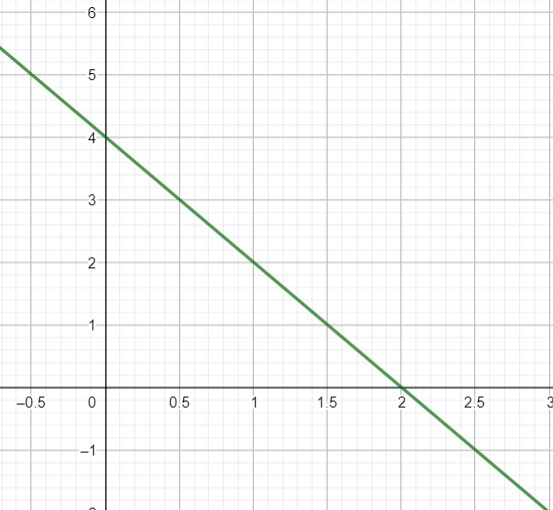
\includegraphics[width=8cm]{Opgave_11-20/Opgave_19/19.jpg}\\\\
Bestem en ligning for linjen.\\\\

\ans
Vi ved at en linje som denne har den generelle form $y = ax + b$. Her er a hældningen og b er skæringen med y-aksen. Vi aflæser skæringen med y-aksen på grafen til $b = 4$. For at bestemme hældningen $a$ skal vi benytte os af følgende formel
\begin{align*}
    a = \frac{y_2-y_1}{x_2-x_1}
\end{align*}
Her er $(x_1,y_1)$ og $(x_2,y_2)$ to vilkårlige punkter på vores linje. For nemhedens skyld vælger vi punkterne til at være 
\begin{align*}
    (x_1,y_1) = (0,4)\\
    (x_2,y_2) = (2,0)
\end{align*}
Indsætter vi disse punkter i formlen bestemmer vi nu a
\begin{align*}
    a = \frac{0-4}{2-0}=\frac{-4}{2}=-2
\end{align*}
Linjens ligning er derfor
\begin{align*}
    y = -2x + 4
\end{align*}